\chapter[第三章]{} % (fold)
\label{cha:chapter3}

\section{3次样条插值函数}

\subsection{问题}

\begin{enumerate}[(1)]
    \item 编制求第一型3次样条插值函数的通用程序;
    \item 已知汽车门曲线型值点的数据如下:

        \begin{table}[ht]\centering
        \begin{tabular}{c|cccccccccccc}
            i & 0 & 1 & 2 & 3 & 4 & 5 & 6 & 7 & 8 & 9 & 10\\
            \hline
            $x_i$ & 0 & 1 & 2 & 3 & 4 & 5 & 6 & 7 & 8 & 9 & 10\\
            $y_i$ & 2.51 & 3.30 & 4.04 & 4.70 & 5.22 & 5.54 & 5.78 & 5.40 & 5.57 & 5.70 & 5.80 
        \end{tabular}
        \end{table}
    
    端点条件为$y_0^{'}=0.8$,$y_{10}^{'}=0.2$,用所编程序求车门的三次样条插值函数$S(x)$,并打印出$S(i+0.5),i=0,1,\cdots,9$。     
\end{enumerate}

\subsection{分析}

根据3次样条插值的定义,插值函数 $S(x)$ 满足:1. $S(x)$ 在每一个小区间上式3次多项式,2. $S(x)$ 在区间 $[a,b]$ 上具有连续2阶导数,3. $S(x)$ 经过每一个给定的插值节点。

在区间 $[a,b]$ 上有 $n+1$ 个插值节点,因此可以设每个小区间上的插值函数 $S_i(x)$ 为:

\begin{equation}
    S_i(x) = a_ix^3  + b_ix^2 + c_ix + d_i
\end{equation}

在 $n$ 个区间上有 $n$ 个插值函数,每个插值函数有 4 个参数,因此需要 $4n$ 个不相关的方程来求解:

\begin{enumerate}[(1)]
    \item 每个插值函数都会经过它所在小区间上的插值节点,即小区间的两个端点,有 $2n$ 个方程:
    \begin{align}
        S_i(x_i) &= y_i, \quad i \in [0,n-1] \\
        S_i(x_{i+1}) &= y_{i+1}, \quad i \in [0,n-1]
    \end{align}

    \item 一阶导数连续,即两个相邻的插值函数连接点处的一阶导数相等,有 $n-1$ 个方程:
    \begin{equation}
        S_i^{'}(x_{i+1}) = S_{i+1}^{'}(x_{i+1}), \quad i \in [0,n-2]
    \end{equation}

    \item 二阶导数连续,即两个相邻的插值函数连接点处的二阶导数相等,有 $n-1$ 个方程:
    \begin{equation}
        S_i^{''}(x_{i+1}) = S_{i+1}^{''}(x_{i+1}), \quad i \in [0,n-2]
    \end{equation}
    
    \item 第一型边界条件,已知两个端点处的一阶导数值,有 2 个方程:
    \begin{align}
        S_0^{'}(x_0) &= y_0^{'} \\
        S_{n-1}^{'}(x_n) &= y_n^{'}
    \end{align}
\end{enumerate}

$4n$ 个方程,使用列主元高斯法求解方程,得到最终的插值函数。

\subsection{程序}

\begin{lstlisting}[style = python]
    import numpy as np
    import matplotlib.pyplot as plt
    from pylab import mpl
    import sys, os
    
    '''
    description: 
    param {*} x n+1 个插值点
    param {*} y n+1 个插值点
    return {*} n
    '''
    def Prejudgment(x, y):
        n1 = len(x)
        n2 = len(y)
        if n1 != n2:
            print('x 与 y 长度不相等')
            sys.exit()
        
        n = n1-1
        return n
            
    '''
    description: 求三次样条差值的 4n 个方程
    param: {x[0,n], y[0,n]} n+1 个插值点
    param: Type 三次样条边界条件 1 or 2 or 3
    return {A, B} [a0 b0 c0 d0 a1 b1 c1 d1 ... a(n-1) b(n-1) c(n-1) d(n-1)] = [B] 形式的方程组 
    '''
    def calculateEquationParameters(x, y, Type=1, dy0=0, dyn=0):
        n = Prejudgment(x, y)
    
        parameterA = []
        parameterB = []
        
        # S_i(x_i) = y_i
        # S_i(x_{i+1}) = y_{i+1}
        # 0 <= i <= n-1
        for i in range(0, n):
            # S_i(x_i) = y_i
            data = np.zeros(n*4)
            data[i*4] = pow(x[i], 3)
            data[i*4+1] = pow(x[i], 2)
            data[i*4+2] = x[i]
            data[i*4+3] = 1
            parameterA.append(data.tolist())
            parameterB.append(y[i])
            
            # S_i(x_{i+1}) = y_{i+1}
            data1 = np.zeros(n*4)
            data1[i*4] = pow(x[(i+1)], 3)
            data1[i*4+1] = pow(x[(i+1)], 2)
            data1[i*4+2] = x[(i+1)]
            data1[i*4+3] = 1
            parameterA.append(data1.tolist())
            parameterB.append(y[i+1])
    
        # S'_i(x_{i+1}) = S'_{i+1}(x_{i+1})
        # 0 <= i <= n-2
        for i in range(0, n-1):
            data = np.zeros(n*4)
    
            data[i*4] = 3 * pow(x[i+1], 2)
            data[i*4+1] = 2 * x[i+1]
            data[i*4+2] = 1
    
            data[(i+1)*4] = -3 * pow(x[i+1], 2)
            data[(i+1)*4+1] = -2 * x[i+1]
            data[(i+1)*4+2] = -1
            
            parameterA.append(data.tolist())
            parameterB.append(0)
    
        # S''_i(x_{i+1}) = S''_{i+1}(x_{i+1})
        # 0 <= i <= n-2
        for i in range(0, n-1):
            data = np.zeros(n*4)
    
            data[i*4] = 6 * x[i+1]
            data[i*4+1] = 2
    
            data[(i+1)*4] = -6 * x[i+1]
            data[(i+1)*4+1] = -2
            
            parameterA.append(data.tolist())
            parameterB.append(0)
    
        if Type == 1:
            # S'_0(x_0) = y'_0
            data = np.zeros(n*4)
            data[0] = 3 * pow(x[0], 2)
            data[1] = 2 * x[0]
            data[2] = 1
            parameterA.append(data.tolist())
            parameterB.append(dy0)
    
            # S'_{n-1}(x_n) = y'_n
            data = np.zeros(n*4)
            data[(n-1)*4] = 3 * pow(x[n], 2)
            data[(n-1)*4+1] = 2 * x[n]
            data[(n-1)*4+2] = 1
    
            parameterA.append(data.tolist())
            parameterB.append(dyn)
        elif Type == 2:
            # S''(a) = S''(b) = 0
    
            # S''_0(x_0) = 0
            data = np.zeros(n*4)
            data[0] = 6 * x[0]
            data[1] = 2
            parameterA.append(data.tolist())
            parameterB.append(0)
    
            # S''_{n-1}(x_n) = 0
            data = np.zeros(n*4)
            data[(n-1)*4] = 6 * x[n]
            data[(n-1)*4+1] = 2
            parameterA.append(data.tolist())
            parameterB.append(0)
    
        elif Type == 3:
            # S'(a) = S'(b) and # S''(a) = S''(b)
            pass
        else:
            print('Error! Unknown "Type" Value!')
    
        return parameterA, parameterB
    
    """
    功能:根据所给参数,计算三次函数的函数值:
    参数:OriginalInterval为原始x的区间, parameters为二次函数的系数,x为自变量
    返回值:为函数的因变量
    """
    def calculate(OriginalInterval, paremeters, x):
        n = int(len(paremeters)/4)
        result=[]
        for data_x in x:
    
            Interval = 0
            if data_x <= OriginalInterval[0]:
                Interval = 0
            elif data_x >= OriginalInterval[-1]:
                Interval = n-1
            else:
                for i in range(0,n):
                    if data_x >= OriginalInterval[i] and data_x < OriginalInterval[i+1]:
                        Interval = i
                        break
    
            result.append(paremeters[Interval*4+0]*data_x*data_x*data_x+paremeters[Interval*4+1]*data_x*data_x+paremeters[Interval*4+2]*data_x+paremeters[Interval*4+3])
        return result
    
    """
    功能:将函数绘制成图像
    参数:data_x,data_y为离散的点.new_data_x,new_data_y为由拉格朗日插值函数计算的值。x为函数的预测值。
    返回值:空
    """
    def Draw(data_x,data_y,new_data_x,new_data_y, title):
            plt.plot(new_data_x, new_data_y, label="拟合曲线", color="black")
            plt.scatter(data_x,data_y, label="离散数据",color="red")
            mpl.rcParams['font.sans-serif'] = ['SimHei']
            mpl.rcParams['axes.unicode_minus'] = False
            plt.title("三次样条函数")
            plt.legend(loc="upper left")
            plt.savefig(os.path.join(os.path.dirname(os.path.abspath(__file__)), title+'.png'), dpi=300)
            plt.show()
    
    def PrintS(parameterX):
        n = int(len(parameterX)/4)
        print('S(x) = ')
        for i in range(0,n):
            print("%.6g & %.6g & %.6g & %.6g \\\\" % (parameterX[i*4], parameterX[i*4+1], parameterX[i*4+2], parameterX[i*4+3]))
        print('\n\n')
            
    def main():
        x = [0,    1,    2,    3,    4,    5,    6,    7,    8,    9,    10]
        y = [2.51, 3.30, 4.04, 4.70, 5.22, 5.54, 5.78, 5.40, 5.57, 5.70, 5.80]
        dy0 = 0.8
        dyn = 0.2  
        parameterA, parameterB = calculateEquationParameters(x, y, 1, dy0, dyn)
        parameterX = MGauss_Caculate(parameterA, parameterB)
    
        PrintS(parameterX)
    
        # 画图
        new_data_x = np.arange(x[0]-0.5, x[-1]+0.6, 0.1)
        new_data_y = calculate(x, parameterX, new_data_x)
        Draw(x, y, new_data_x, new_data_y, '三次样条插值')
    
        # 打印
        new_data_x = np.arange(0.5, 10.5, 1)
        new_data_y = calculate(x, parameterX, new_data_x)
        # f4_5 = calculate(parameterX[8:12], [4.5])
        print(new_data_x)
        for i,data in enumerate(new_data_y):
            print("%.6g & " % data)
    
    if __name__ == "__main__":
    
        # 获取当前文件路径
        current_path = os.path.abspath(__file__)
        sys.path.append(os.path.abspath(os.path.join(os.path.dirname(current_path), '../')))
        # print(sys.path)
        # 调用 chapter3 中的列主元高斯消去法
        from chapter3.q3 import MGauss_Caculate
    
        main()
\end{lstlisting}

\subsection{算例}

对题目中的数据进行三次样条插值:

\begin{table}[ht]\centering
    \begin{tabular}{c|cccccccccccc}
        i & 0 & 1 & 2 & 3 & 4 & 5 & 6 & 7 & 8 & 9 & 10\\
        \hline
        $x_i$ & 0 & 1 & 2 & 3 & 4 & 5 & 6 & 7 & 8 & 9 & 10\\
        $y_i$ & 2.51 & 3.30 & 4.04 & 4.70 & 5.22 & 5.54 & 5.78 & 5.40 & 5.57 & 5.70 & 5.80 
    \end{tabular}
\end{table}

得到的插值函数系数为:

$$
\begin{bmatrix}
    -0.00851404 & -0.00148596 & 0.8 & 2.51 \\
    -0.00445789 & -0.0136544 & 0.812168 & 2.50594 \\
    -0.00365441 & -0.0184753 & 0.82181 & 2.49952 \\
    -0.0409245 & 0.316955 & -0.184482 & 3.50581 \\
    0.107352 & -1.46237 & 6.93281 & -5.98391 \\
    -0.268485 & 4.17519 & -21.255 & 40.9958 \\
    0.426587 & -8.33611 & 53.8128 & -109.14 \\
    -0.267865 & 6.24739 & -48.2717 & 129.057 \\
    0.0548723 & -1.4983 & 13.6939 & -36.1842 \\
    0.0583759 & -1.5929 & 14.5453 & -38.7383 \\
\end{bmatrix}
$$

题目中要求的 $S(i+0.5),i=0,1,\cdots,9$ 值如表\ref{tab:Si}所示,插值函数的图像如图\ref{fig:spline}所示。

\begin{table}[ht]\centering
\caption{$S(i+0.5),i=0,1,\cdots,9$}
\label{tab:Si}
    \begin{tabular}{c|cccccccccccc}
        i & 0 & 1 & 2 & 3 & 4 \\
        \hline
        $x_i$ & 0.5 & 1.5 & 2.5 & 3.5 & 4.5 \\
        $S(x)$ & 2.90856 & 3.67843 & 4.38147 & 4.98819 & 5.38328 \\
        \hline\hline
        i & 5 & 6 & 7 & 8 & 9 \\
        \hline
        $x_i$ & 5.5 & 6.5 & 7.5 & 8.5 & 9.5\\
        $S(x)$ & 5.7237 & 5.59441 & 5.42989 & 5.65977 & 5.7323 
    \end{tabular}
\end{table}

\begin{figure}[ht]
    \centering
      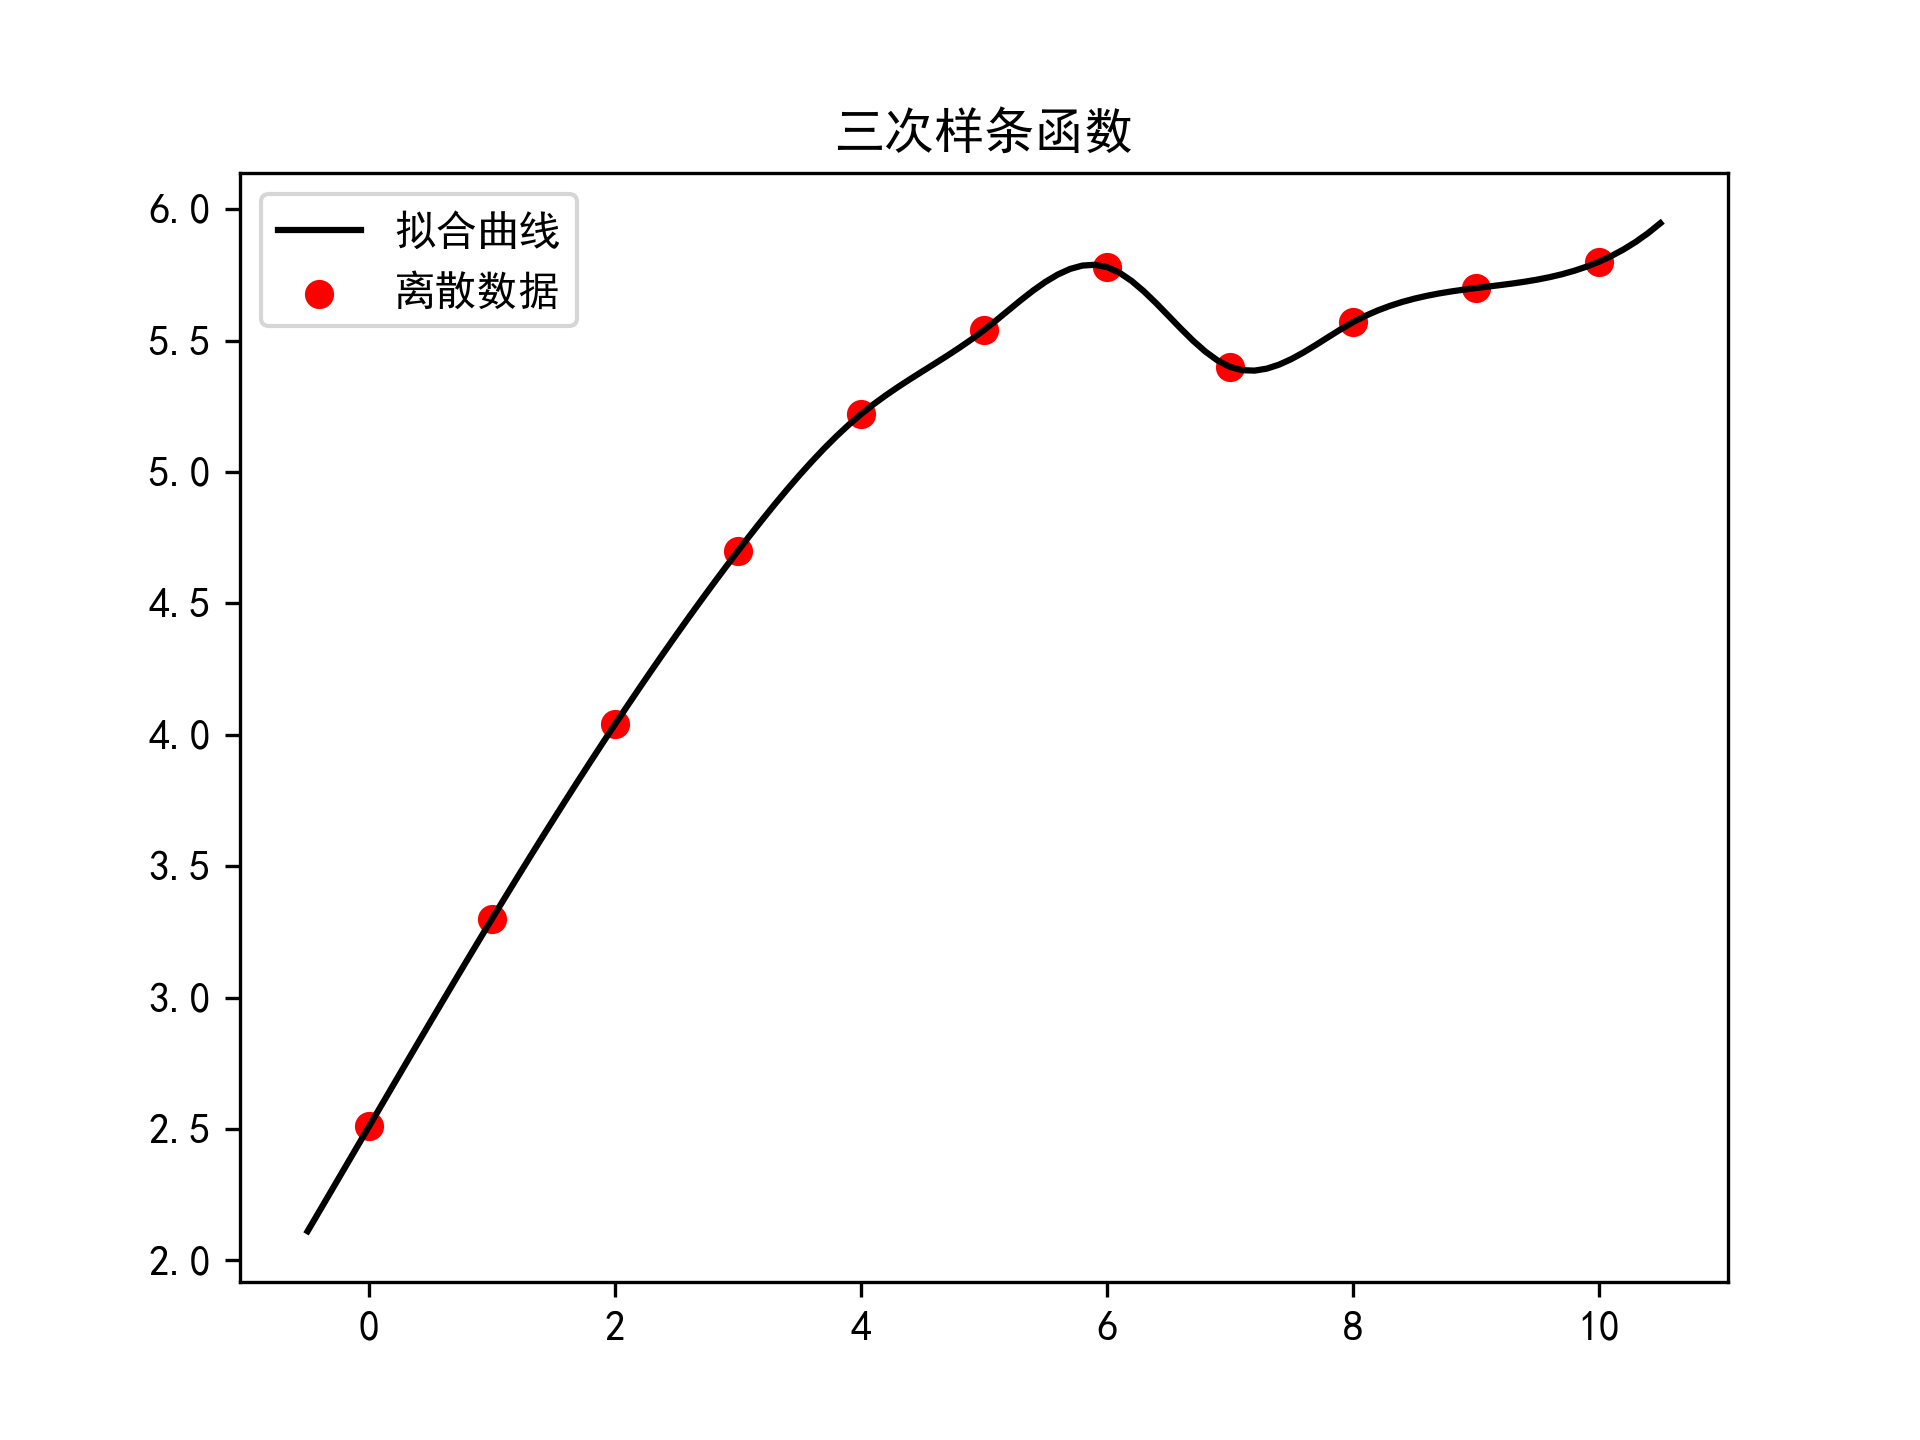
\includegraphics[width=\textwidth]{spline}
      \caption{三次样条插值图像}
      \label{fig:spline}
\end{figure}


\subsection{结论}

\begin{enumerate}[(1)]
    \item 编写程序实现了第一型边界条件和第二型边界条件下的三次样条插值计算;
    \item 三次样条插值得到的函数二阶导数连续,因此其光滑性较好;
    \item 目前算法使用的是待定系数法求解,当插值节点较多时,计算量较大,应加以改进。
\end{enumerate}

\clearpage

\section{离散数据的最佳平方逼近}

\subsection{问题}

一种商品的需求量和其价格有一定关系,先对一定时期内的商品价格 x 与需求量 y 进行观察,取得如下的样本数据,如表\ref{tab:sample_data}所示。

\begin{table}[ht]\centering
    \caption{样本数据}
    \label{tab:sample_data}
    \begin{tabular}{c|cccccccccccc}
        价格 & 2 & 3 & 4 & 5 & 6 & 7 & 8 & 9 & 10 & 11 \\
        \hline
        需求量 & 58 & 50 & 44 & 38 & 34 & 30 & 29 & 26 & 25 & 24
    \end{tabular}
\end{table}

\begin{enumerate}[(1)]
    \item 对上述数据,分别求出其 2, 3, 4 次最佳平方逼近多项式。画出图形,并比较拟合误差:
    \begin{equation}
        Q = \sum\limits_{k=1}^{n}(q(x_k) - y_k)^2
    \end{equation}
    \item 假设拟合函数分别为:
    \begin{equation}
        a+\frac{b}{x},\quad a+b\mathrm{ln}x, \quad ae^{bx},\quad \frac{1}{a+bx}
    \end{equation}
    分别求出 a, b 的值。绘图,计算误差,并比较优劣。
\end{enumerate}

\subsection{分析}

本题是一个离散数据的最佳平方逼近问题,对于这类问题,首先要将拟合函数化为标准形式,即 $p(x)=\sum\limits_{k=1}^{n}(c_i \varphi_i(x))$,然后求出正规方程,通过求解正规方程得到拟合函数系数 $c_i$,如有需要再将标准形式的拟合函数化为需要的形式。

在第二问中,四个拟合函数都不是标准形式。

\begin{enumerate}
    \item 对于 $y=a+{b}/{x}$,令 $t = 1/x$,则 $y = a+bt$;
    \item 对于 $y=a+b\mathrm{ln}x$,令 $t = \mathrm{ln}x$,则 $y = a+bt$;
    \item 对于 $y=ae^{bx}$,两边取对数,得到 $\mathrm{ln}y = \mathrm{ln}a + bx$;
    \item 对于 $y={1}/(a+bx)$,令 $t = 1/y$,则 $t = a+bx$。
\end{enumerate}

\subsection{程序}

\begin{lstlisting}[style = python]
    # 离散数据的最佳平方逼近
    import numpy as np
    import sys, os
    import matplotlib.pyplot as plt
    from pylab import mpl
    import math

    '''
    description: 
    param {*} x n+1 个插值点
    param {*} y n+1 个插值点
    return {*} n
    '''
    def PrejudgmentShape(x, y):
        n1 = len(x)
        n2 = len(y)
        if n1 != n2:
            print('x 与 y 长度不相等')
            sys.exit()
        
        n = n1-1
        return n

    '''
    description: 求最佳平方逼近的正规方程
    param {*} m m次最佳平方逼近
    param {*} x n个自变量x
    param {*} y n个因变量y
    return {*} (A, b)
    '''
    def GetNormalEquation(m, x, y):
        A = []
        b = []
        PrejudgmentShape(x, y)
        for j in range(0,m+1):
            AAline = []
            for i in range(0, m+1):
                tmp = np.dot(np.power(x, j), np.power(x, i))
                AAline.append(tmp)
            A.append(AAline)
            tmp = np.dot(y, np.power(x, j))
            b.append(tmp)
        return A, b

    '''
    description: 获取最佳平方逼近的多项式
    param {*} A 正规方程系数A
    param {*} b 正规方程系数b
    return {*} c 多项式系数,q(x) = c0 + c1*x + c2*x^2 + ... + cm*x^m
    '''
    def GetExpression(A, b):
        c = MGauss_Caculate(A, b)
        return c

    '''
    description: 计算最佳平方逼近多项式
    param {*} m m次最佳平方逼近
    param {*} x n个自变量x
    param {*} y n个因变量y
    return {*} c 最佳平方逼近多项式系数,q(x) = c0 + c1*x + c2*x^2 + ... + cm*x^m
    '''
    def GetLeastSquaresApproximationExpression(m, x, y):
        A, b = GetNormalEquation(m, x, y)
        c = GetExpression(A, b)
        return c

    '''
    description: 计算多项式,q(x) = c0 + c1*x + c2*x^2 + ... + cm*x^m
    param {*} c 最佳平方逼近多项式系数
    return {*} 多项式结果
    '''
    def CaculateExpression(c, x):
        res = 0
        for i, ci in enumerate(c):
            res = res + ci * pow(x, i)
        return res

    '''
    description: 计算多项式, x form x0 to xn, q(x) = c0 + c1*x + c2*x^2 + ... + cm*x^m
    param {*} c 最佳平方逼近多项式系数
    param {list} xn 
    return {*}
    '''
    def CaculateInterval(c, xn):
        res = []
        for x in xn:
            res.append(CaculateExpression(c, x))
        return res

    """
    功能:将函数绘制成图像
    参数:data_x, data_y 为原始值,new_data_x, new_data_y 为预测计算的值。
    返回值:空
    """
    def Draw(data_x,data_y,new_data_x,new_data_y, title):
        plt.plot(new_data_x, new_data_y, label="拟合曲线", color="black")
        plt.scatter(data_x,data_y, label="离散数据",color="red")
        mpl.rcParams['font.sans-serif'] = ['SimHei']
        mpl.rcParams['axes.unicode_minus'] = False
        plt.title(title)
        plt.legend(loc="upper right")
        plt.savefig(os.path.join(os.path.dirname(os.path.abspath(__file__)), title+'.png'), dpi=300)
        plt.show()

    '''
    description: 计算拟合误差 Q = \Sigma_{k=1}^{n} (q(x_k) - y_k)^2 
    param {*} c 最佳平方逼近多项式系数, q(x) = c0 + c1*x + c2*x^2 + ... + cm*x^m
    param {*} x
    param {*} y
    return {*} Q
    '''
    def GetFittingError(c, x, y):
        Err = 0
        for n, xn in enumerate(x):
            qx = CaculateExpression(c, xn)
            Err += pow((qx - y[n]), 2)
        return Err

    '''
    description: 别求出其 2, 3, 4 次最佳平方逼近多项式.画出图形, 并比较拟合误差
    param {*}
    return {*}
    '''
    def Q1():
        x = [2, 3, 4, 5, 6, 7, 8, 9, 10, 11]
        y = [58, 50, 44, 38, 34, 30, 29, 26, 25, 24]

        result_file = os.path.join(os.path.dirname(os.path.abspath(__file__)), '最佳平方逼近_result.txt')

        if os.path.exists(result_file):
            os.remove(result_file)
        
        # 最佳平方逼近
        for m in range(2, 5):
            c = GetLeastSquaresApproximationExpression(m, x, y)
            # 画图
            new_x = np.arange(x[0]-0.5, x[-1]+0.6, 0.1)
            new_y = CaculateInterval(c, new_x)
            Draw(x, y, new_x, new_y, "{0}次最佳平方逼近".format(m))
            # 拟合误差
            FittingErr = GetFittingError(c, x, y)
            # 写入文件
            with open(result_file, "a+") as fo:
                fo.write("\n\\********************************************************\\\n")
                fo.write("{0} 次最佳平方逼近, m = {1}\n".format(m, m))
                fo.write("x = ")
                for xi in x:
                    fo.write(str(xi))
                    fo.write("\t")
                fo.write("\n")
                fo.write("y = ")
                for yi in y:
                    fo.write(str(yi))
                    fo.write("\t")
                fo.write("\n")
                fo.write("近似函数:q(x) = c0 + c1*x + c2*x^2 + ... + cm*x^m \n")
                fo.write("c = ")
                for ci in c:
                    fo.write(str(format(ci, '.6g')))
                    fo.write("\t")
                fo.write("\n")
                fo.write("拟合误差:{0}\n".format(format(FittingErr, '.8g')))
                fo.write("\\********************************************************\\\n")

    # a+b÷x近似
    def Q2_1():
        x = [2, 3, 4, 5, 6, 7, 8, 9, 10, 11]
        y = [58, 50, 44, 38, 34, 30, 29, 26, 25, 24]

        result_file = os.path.join(os.path.dirname(os.path.abspath(__file__)), 'a+b÷x近似_result.txt')

        # a + b/x
        x1 = [1.0/xi for xi in x]
        c = GetLeastSquaresApproximationExpression(1, x1, y)
        # 画图
        new_x = np.arange(x[0]-0.5, x[-1]+0.6, 0.1)
        new_x1 = [1.0/xi for xi in new_x]
        new_y = CaculateInterval(c, new_x1)
        Draw(x, y, new_x, new_y, "a+b÷x近似")
        # 拟合误差
        FittingErr = GetFittingError(c, x1, y)
        # 写入文件
        with open(result_file, "w+") as fo:
            fo.write("\n\\********************************************************\\\n")
            fo.write("a+b÷x近似\n")
            fo.write("x = ")
            for xi in x:
                fo.write(str(xi))
                fo.write("\t")
            fo.write("\n")
            fo.write("y = ")
            for yi in y:
                fo.write(str(yi))
                fo.write("\t")
            fo.write("\n")
            fo.write("近似函数:q(x) = {} + {} / x \n".format(c[0], c[1]))
            fo.write("拟合误差:{0}\n".format(FittingErr))
            fo.write("\\********************************************************\\\n")

    # a+blnx近似
    def Q2_2():
        x = [2, 3, 4, 5, 6, 7, 8, 9, 10, 11]
        y = [58, 50, 44, 38, 34, 30, 29, 26, 25, 24]

        result_file = os.path.join(os.path.dirname(os.path.abspath(__file__)), 'a+blnx近似_result.txt')

        # a + blnx
        x1 = [math.log(xi) for xi in x]
        c = GetLeastSquaresApproximationExpression(1, x1, y)
        # 画图
        new_x = np.arange(x[0]-0.5, x[-1]+0.6, 0.1)
        new_x1 = [math.log(xi) for xi in new_x]
        new_y = CaculateInterval(c, new_x1)
        Draw(x, y, new_x, new_y, "a+blnx近似")
        # 拟合误差
        FittingErr = GetFittingError(c, x1, y)
        # 写入文件
        with open(result_file, "w+") as fo:
            fo.write("\n\\********************************************************\\\n")
            fo.write("a+blnx近似\n")
            fo.write("x = ")
            for xi in x:
                fo.write(str(xi))
                fo.write("\t")
            fo.write("\n")
            fo.write("y = ")
            for yi in y:
                fo.write(str(yi))
                fo.write("\t")
            fo.write("\n")
            fo.write("近似函数:q(x) = {} + {} ln(x) \n".format(c[0], c[1]))
            fo.write("拟合误差:{0}\n".format(FittingErr))
            fo.write("\\********************************************************\\\n")

    '''
    description: 计算拟合误差 Q = \Sigma_{k=1}^{n} (q(x_k) - y_k)^2 
    param {*} c 最佳平方逼近多项式系数, q(x) = a*exp(bx)
    param {*} x
    param {*} y
    return {*} Q
    '''
    def GetFittingError_q2_3(c, x, y):
        Err = 0
        for n, xn in enumerate(x):
            qx1 = CaculateExpression(c, xn)
            qx = math.exp(qx1)
            Err += pow((qx - y[n]), 2)
        return Err

    # a*exp(bx)近似
    def Q2_3():
        x = [2, 3, 4, 5, 6, 7, 8, 9, 10, 11]
        y = [58, 50, 44, 38, 34, 30, 29, 26, 25, 24]

        result_file = os.path.join(os.path.dirname(os.path.abspath(__file__)), 'a*exp(bx)近似_result.txt')

        # a + blnx
        y1 = [math.log(yi) for yi in y]
        c = GetLeastSquaresApproximationExpression(1, x, y1)
        # 画图
        new_x = np.arange(x[0]-0.5, x[-1]+0.6, 0.1)
        new_y1 = CaculateInterval(c, new_x)
        new_y = [math.exp(yi) for yi in new_y1]
        Draw(x, y, new_x, new_y, "a*exp(bx)近似")
        # 拟合误差
        FittingErr = GetFittingError_q2_3(c, x, y)
        # 写入文件
        with open(result_file, "w+") as fo:
            fo.write("\n\\********************************************************\\\n")
            fo.write("a*exp(bx)近似\n")
            fo.write("x = ")
            for xi in x:
                fo.write(str(xi))
                fo.write("\t")
            fo.write("\n")
            fo.write("y = ")
            for yi in y:
                fo.write(str(yi))
                fo.write("\t")
            fo.write("\n")
            fo.write("近似函数:q(x) = {0} * exp({1} * x) \n".format(math.exp(c[0]), c[1]))
            fo.write("拟合误差:{0}\n".format(FittingErr))
            fo.write("\\********************************************************\\\n")

    '''
    description: 计算拟合误差 Q = \Sigma_{k=1}^{n} (q(x_k) - y_k)^2 
    param {*} c 最佳平方逼近多项式系数, q(x) = 1/(a+bx)
    param {*} x
    param {*} y
    return {*} Q
    '''
    def GetFittingError_q2_4(c, x, y):
        Err = 0
        for n, xn in enumerate(x):
            qx1 = CaculateExpression(c, xn)
            qx = 1.0/qx1
            Err += pow((qx - y[n]), 2)
        return Err

    # 1÷(a+bx)近似
    def Q2_4():
        x = [2, 3, 4, 5, 6, 7, 8, 9, 10, 11]
        y = [58, 50, 44, 38, 34, 30, 29, 26, 25, 24]

        result_file = os.path.join(os.path.dirname(os.path.abspath(__file__)), '1÷(a+bx)近似_result.txt')

        # a + blnx
        y1 = [1.0/yi for yi in y]
        c = GetLeastSquaresApproximationExpression(1, x, y1)
        # 画图
        new_x = np.arange(x[0]-0.5, x[-1]+0.6, 0.1)
        new_y1 = CaculateInterval(c, new_x)
        new_y = [1.0/yi for yi in new_y1]
        Draw(x, y, new_x, new_y, "1÷(a+bx)近似")
        # 拟合误差
        FittingErr = GetFittingError_q2_4(c, x, y)
        # 写入文件
        with open(result_file, "w+") as fo:
            fo.write("\n\\********************************************************\\\n")
            fo.write("1÷(a+bx)近似\n")
            fo.write("x = ")
            for xi in x:
                fo.write(str(xi))
                fo.write("\t")
            fo.write("\n")
            fo.write("y = ")
            for yi in y:
                fo.write(str(yi))
                fo.write("\t")
            fo.write("\n")
            fo.write("近似函数:q(x) = 1 ÷ ( {0} + {1} * x) \n".format(math.exp(c[0]), c[1]))
            fo.write("拟合误差:{0}\n".format(FittingErr))
            fo.write("\\********************************************************\\\n")

    def main():
        Q1()
        Q2_1()
        Q2_2()
        Q2_3()
        Q2_4()

    if __name__ == "__main__":

        # 获取当前文件路径
        current_path = os.path.abspath(__file__)
        sys.path.append(os.path.abspath(os.path.join(os.path.dirname(current_path), '../')))
        # print(sys.path)
        # 调用 chapter3 中的列主元高斯消去法
        from chapter3.q3 import MGauss_Caculate

        main()
\end{lstlisting}

\subsection{算例}

对于题目中的第一问,分别求出 2, 3, 4 次最佳平方逼近多项式的拟合函数如下,拟合误差分别为 $3.2166667,1.5102564,1.4679487$,拟合函数的图像如图\ref{fig:lsa}所示。

\begin{align}
    p(x) &= 74.3258 -9.31136*x + 0.435606*x^2 \\
    p(x) &= 78.5424 - 11.9462*x + 0.893939*x^2 -0.0235043*x^3 \\
    p(x) &= 76.9924 - 10.6129*x + 0.520542*x^2 + 0.0181624*x^3 -0.00160256*x^4
\end{align}

\begin{figure}[htbp]
    \centering
    \subfigure[2次最佳平方逼近]{
        \begin{minipage}[t]{0.5\linewidth}
        \centering
        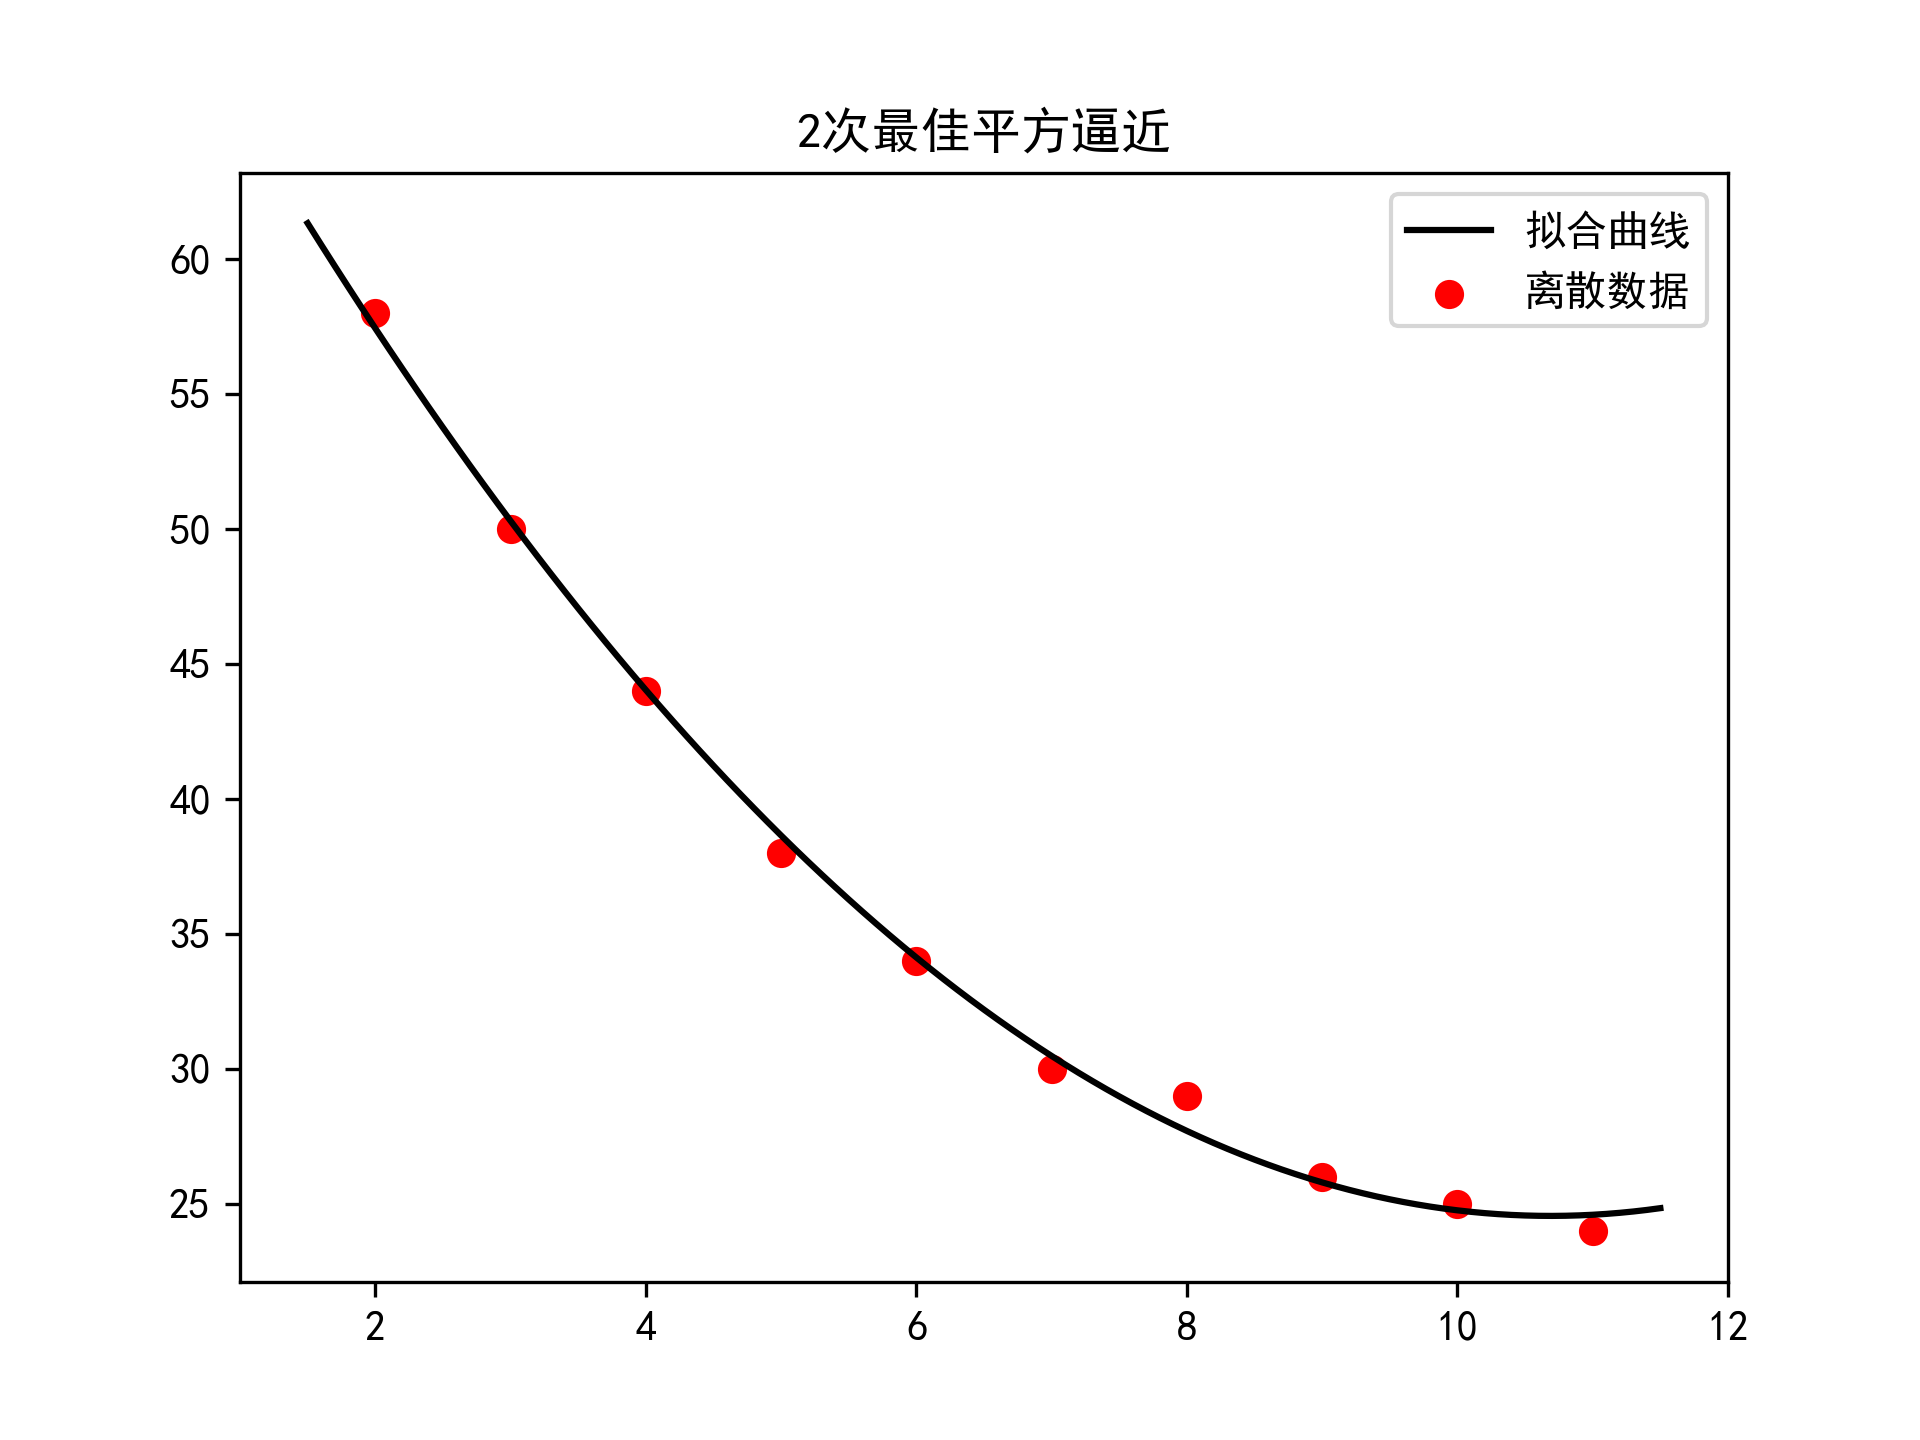
\includegraphics[width=\linewidth]{lsa2}
        %\caption{fig1}
        \end{minipage}%
    }%
    \subfigure[3次最佳平方逼近]{
        \begin{minipage}[t]{0.5\linewidth}
        \centering
        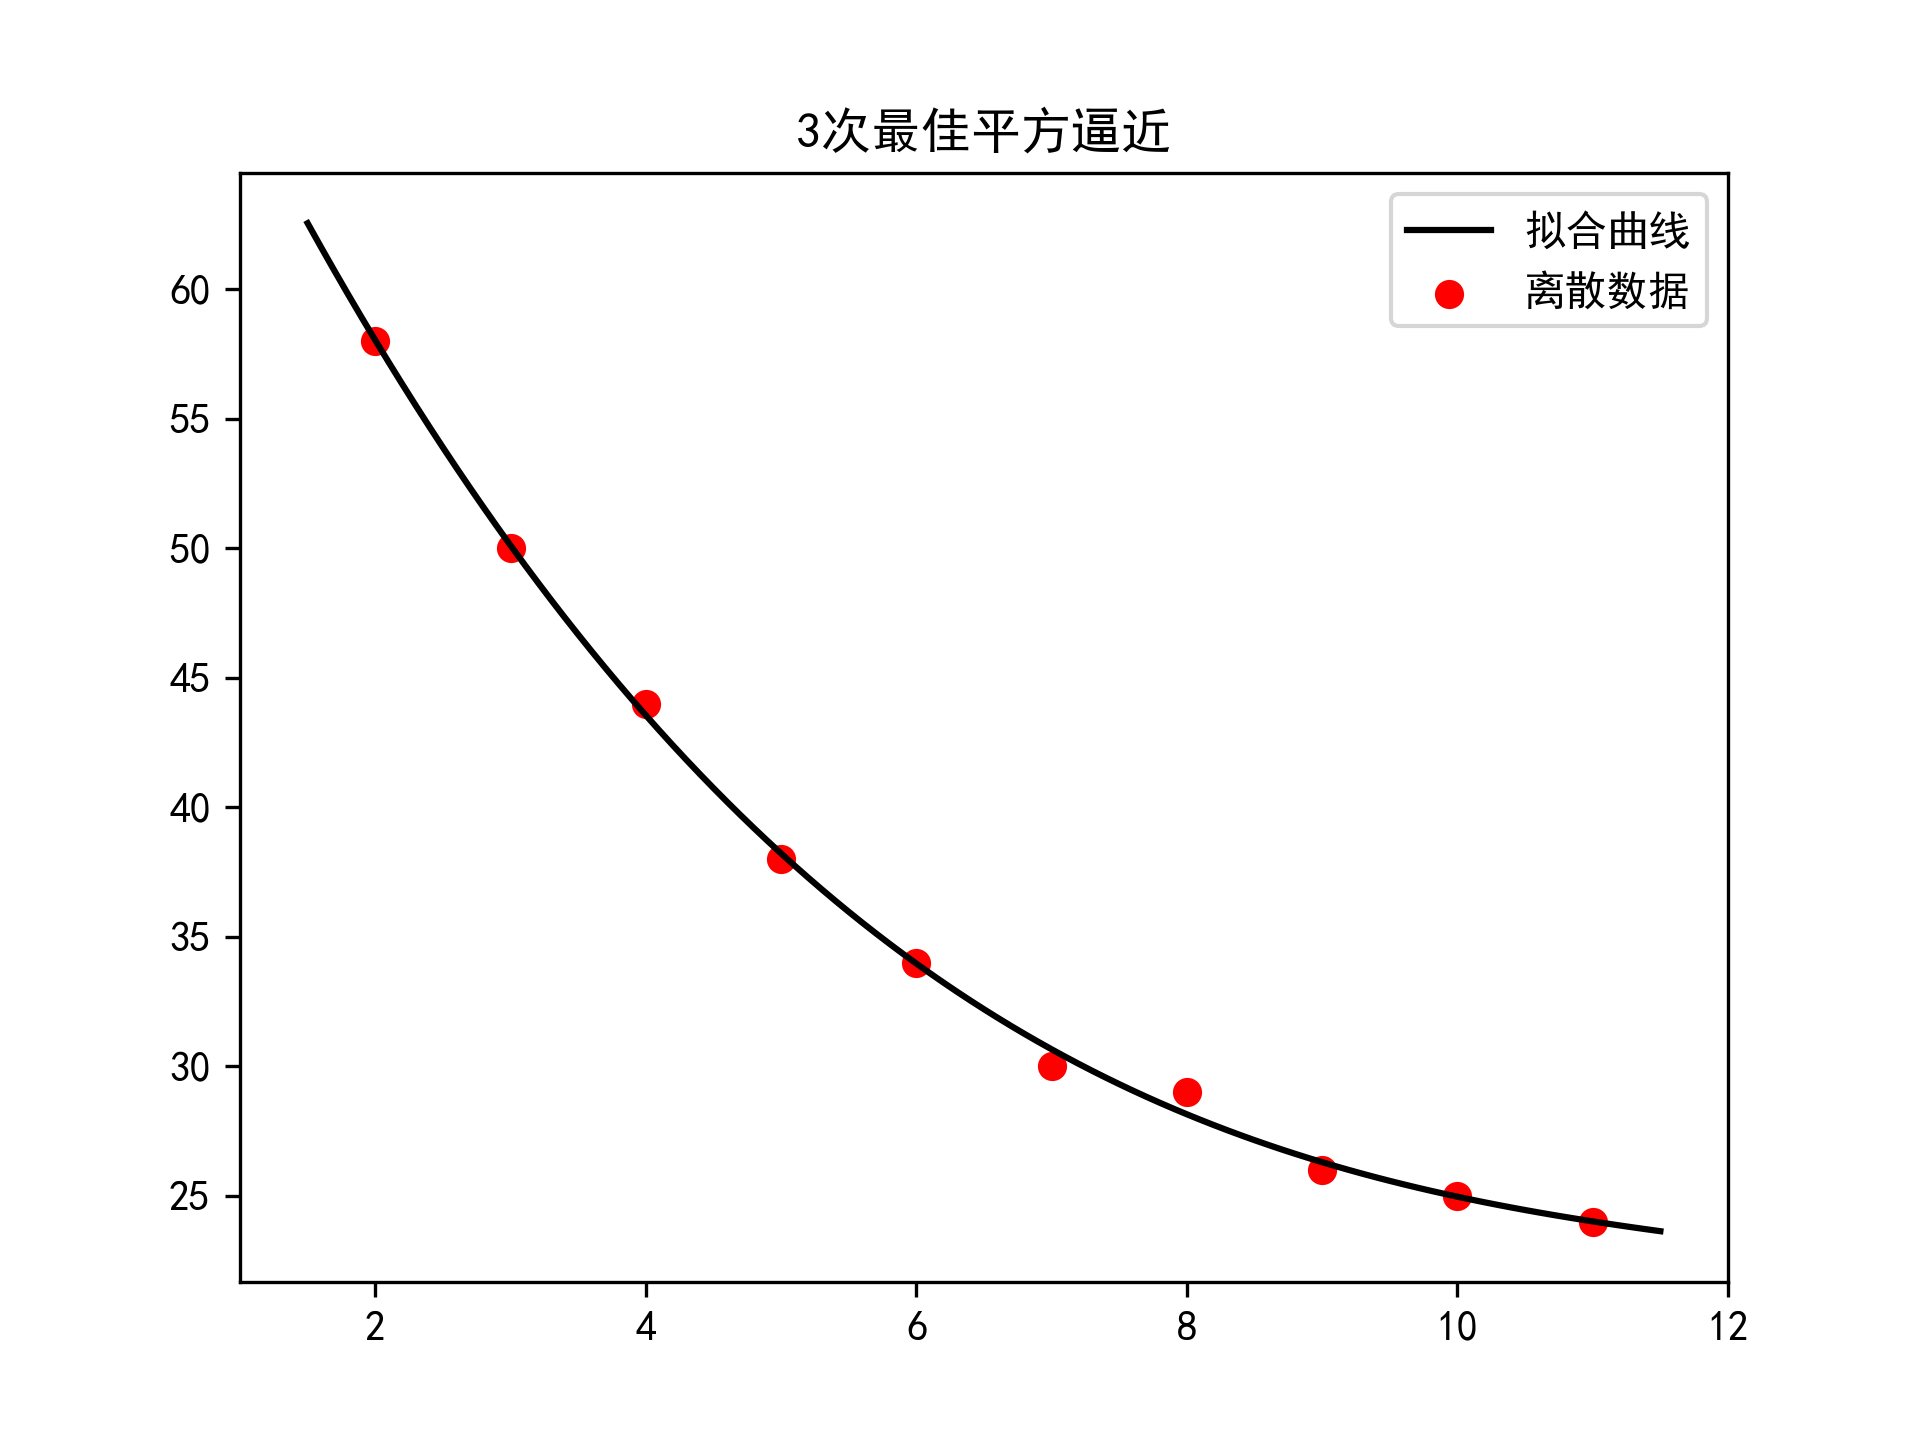
\includegraphics[width=\linewidth]{lsa3}
        %\caption{fig2}
        \end{minipage}%
    }%

    \subfigure[4次最佳平方逼近]{
        \begin{minipage}[t]{0.5\linewidth}
        \centering
        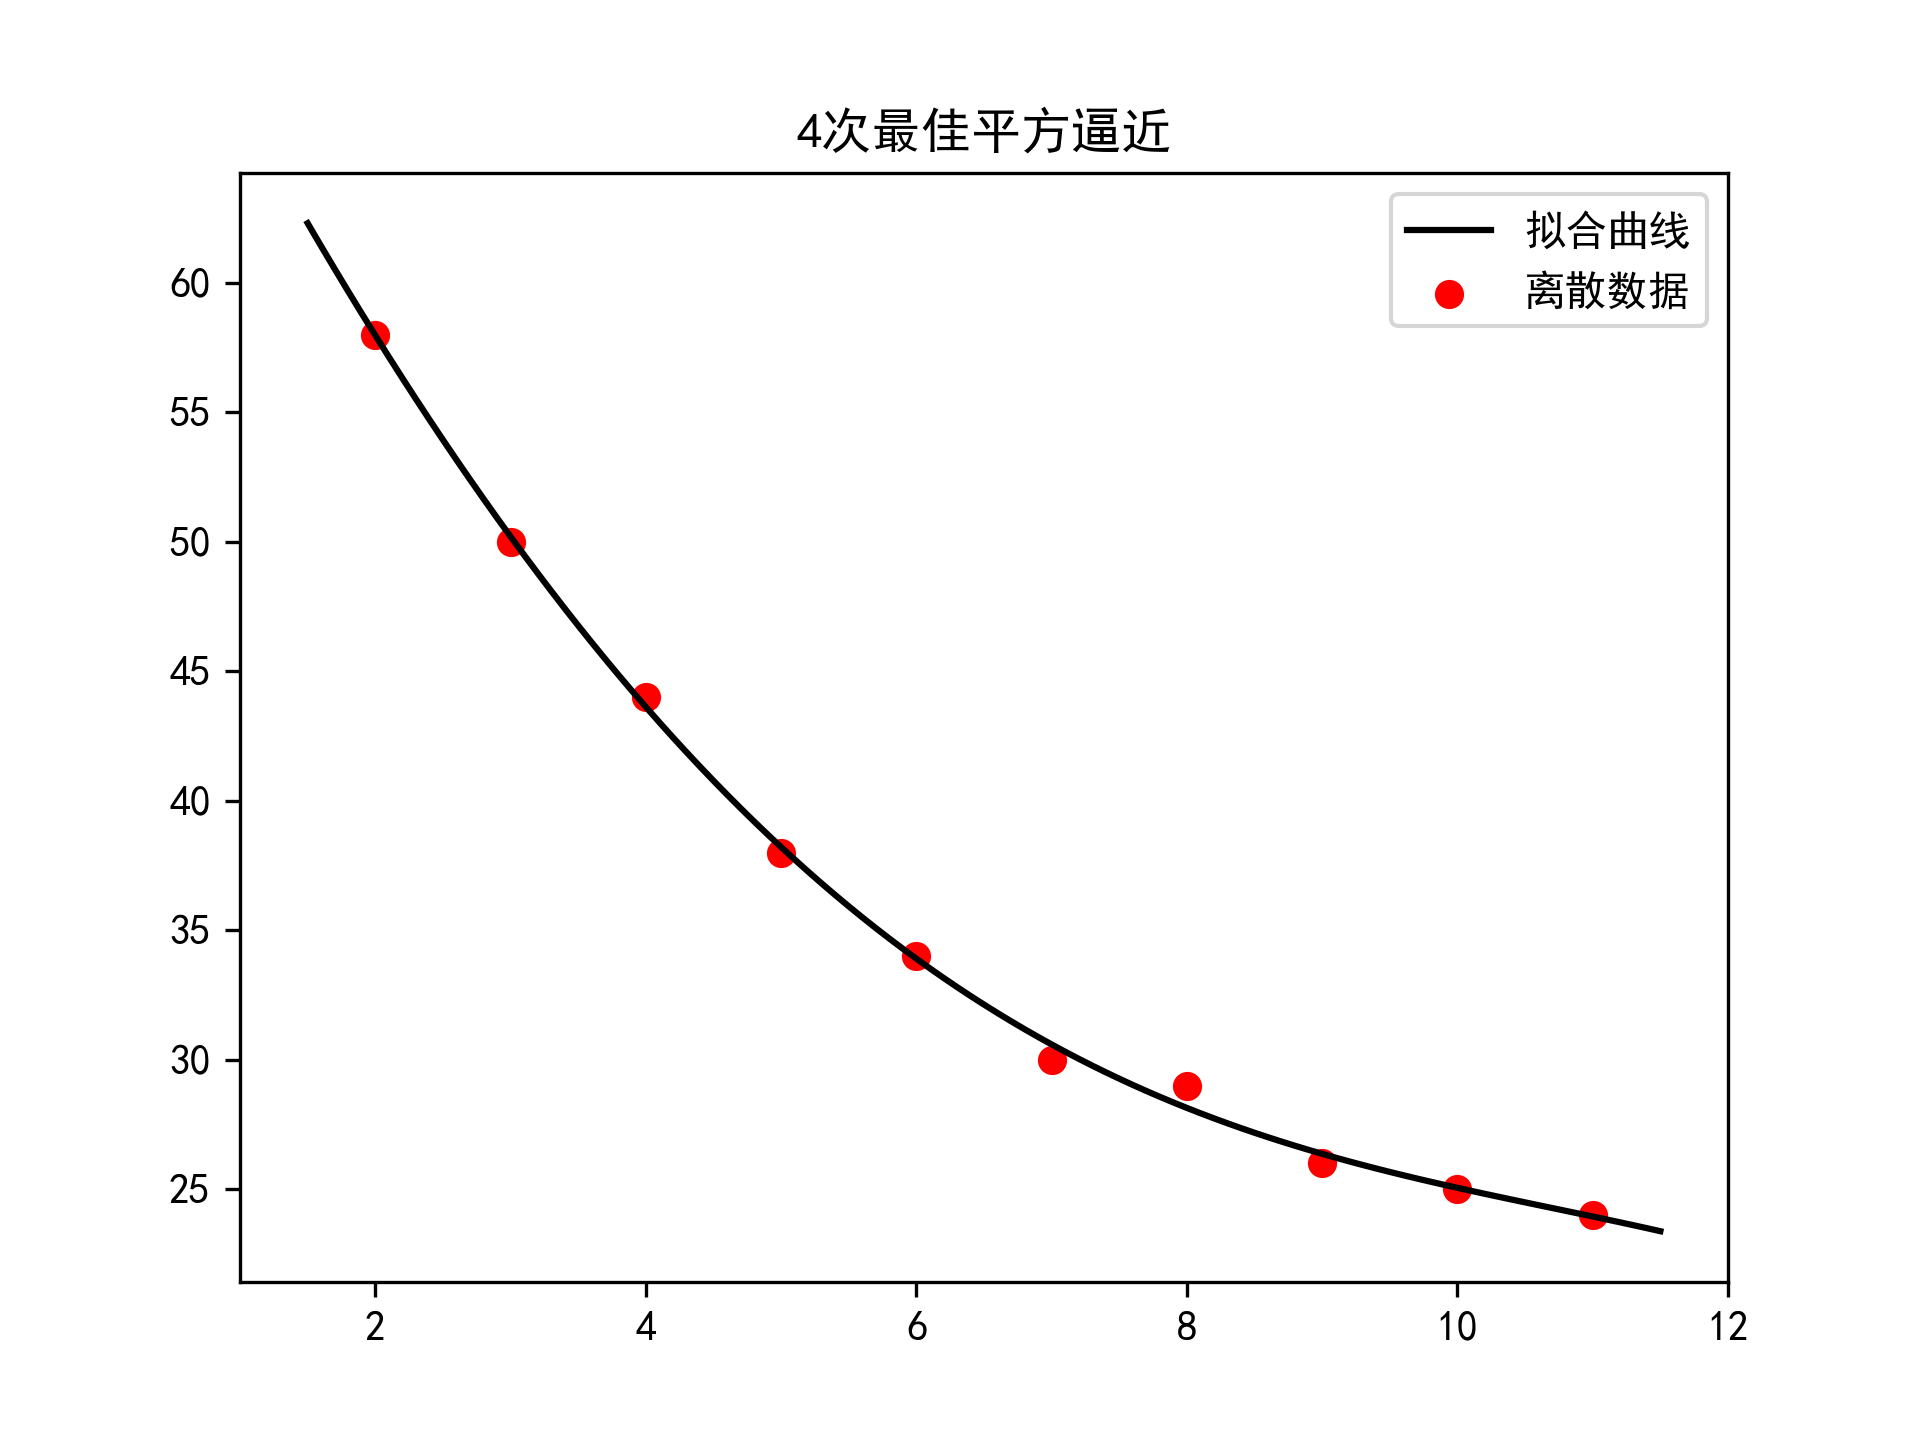
\includegraphics[width=\linewidth]{lsa4}
        %\caption{fig2}
        \end{minipage}
    }%
    \centering
    \caption{最佳平方逼近}
    \label{fig:lsa}
\end{figure}


对于题目中的第二问,拟合函数如下,拟合的图像如图\ref{fig:lsa2}所示,拟合误差分别为 $57.302270,8.7788712,41.844596,7.7324292$。

\begin{align}
    q(x) &= 18.160410958809152 + \frac{87.330000932616}{x}  \\
    q(x) &= 72.13901063630205 -20.762410852503 ln(x)  \\
    q(x) &= 65.29387947714481 * e^{-0.09915171210523323 * x} \\
    q(x) &= \frac{1}{ 1.012042106641784 + 0.0028298266117981353 * x}
\end{align}

\begin{figure}[htbp]
    \centering
    \subfigure[$y=a+{b}/{x}$]{
        \begin{minipage}[t]{0.5\linewidth}
        \centering
        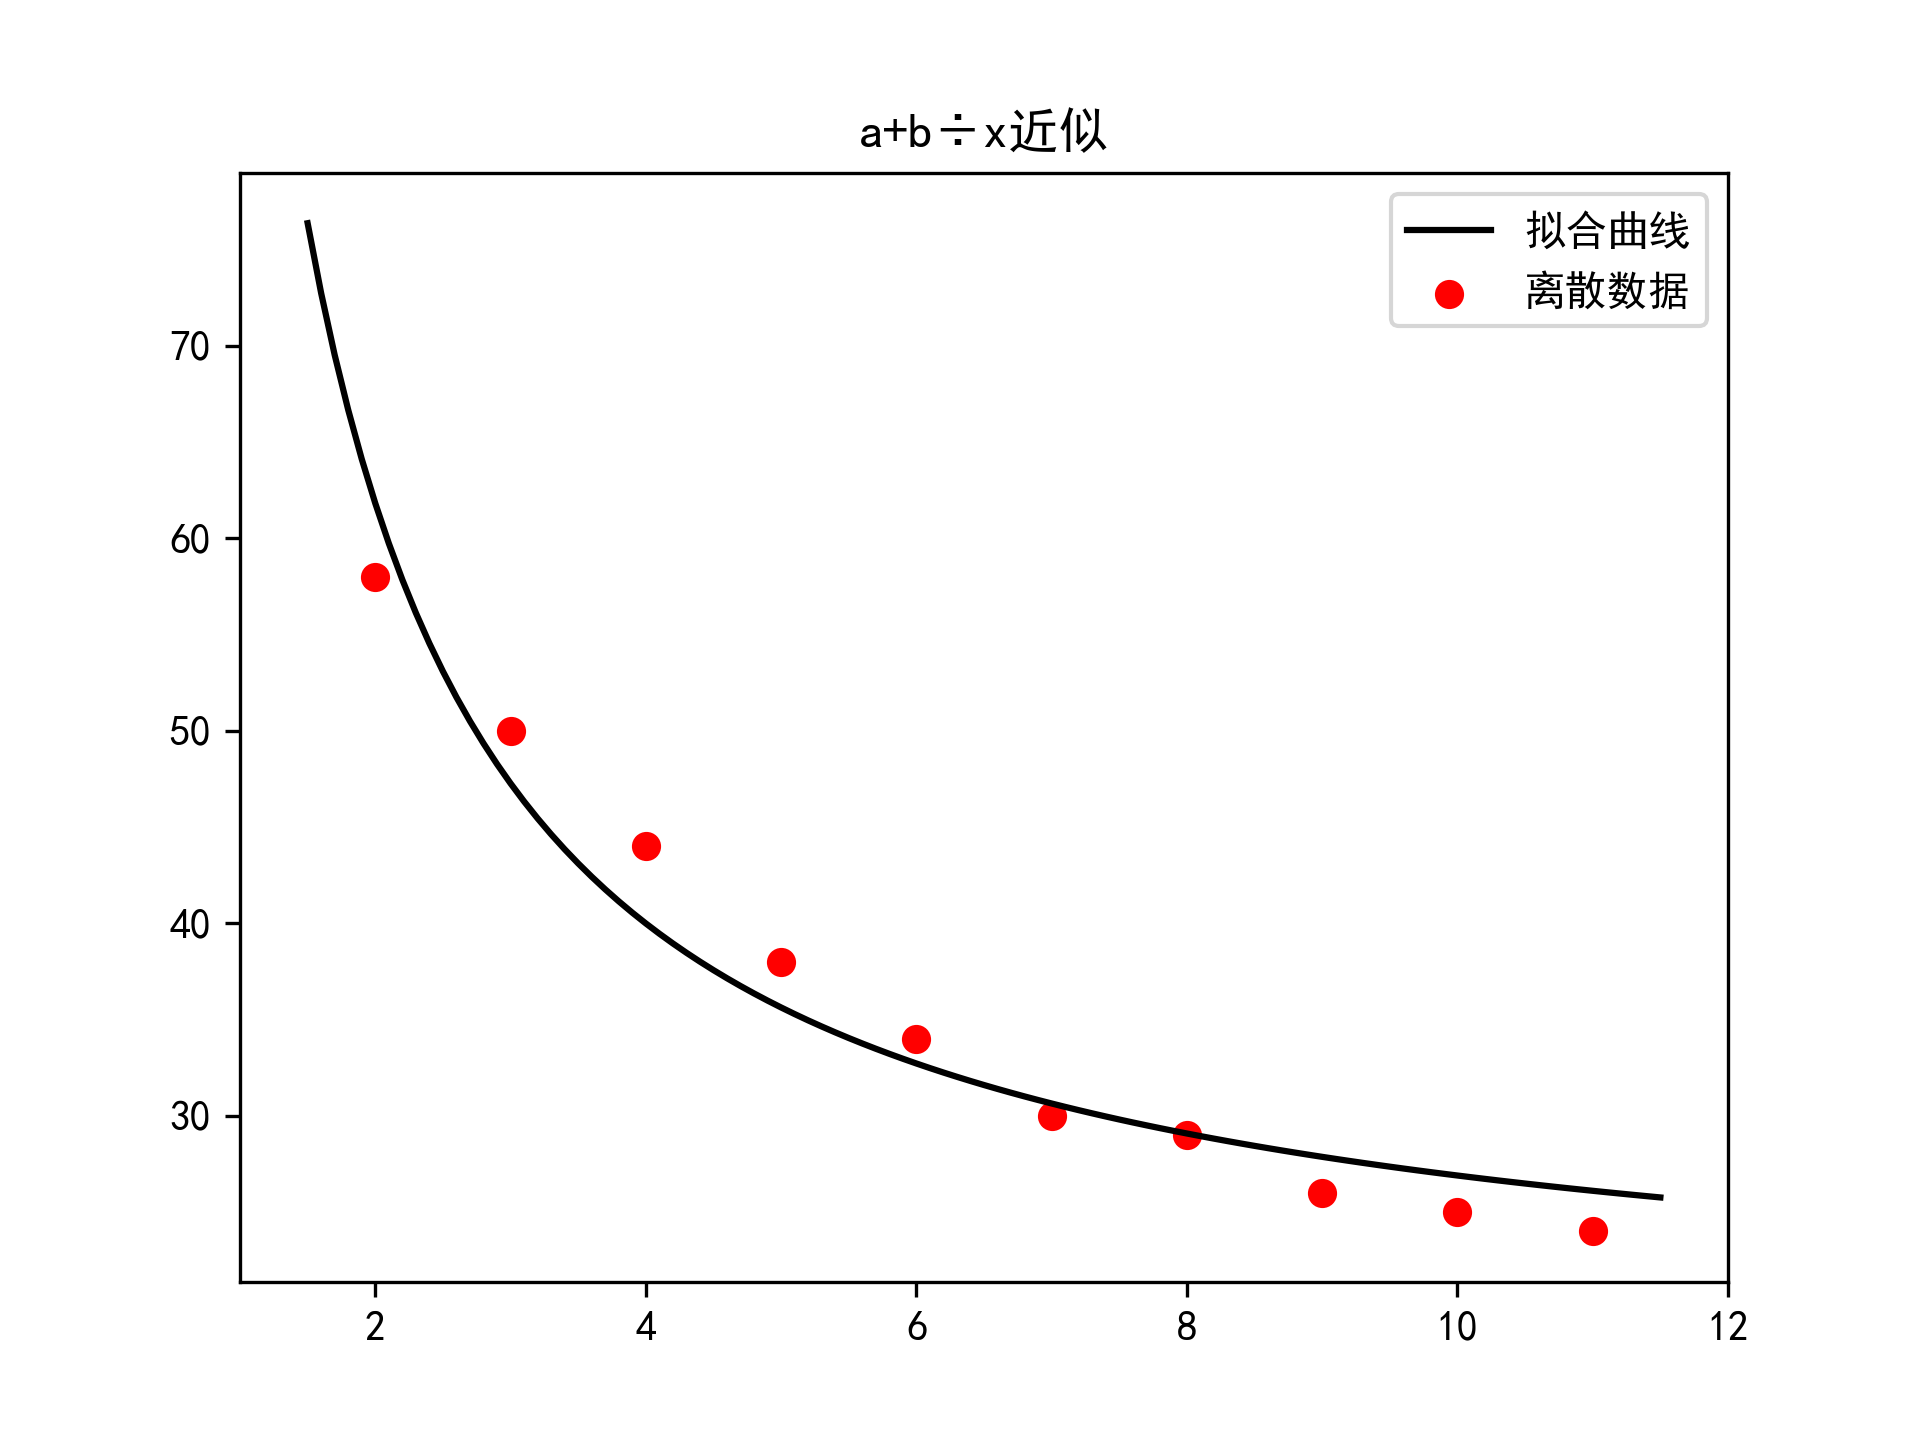
\includegraphics[width=\linewidth]{a+b÷x近似}
        %\caption{fig1}
        \end{minipage}%
    }%
    \subfigure[$y=a+b\mathrm{ln}x$]{
        \begin{minipage}[t]{0.5\linewidth}
        \centering
        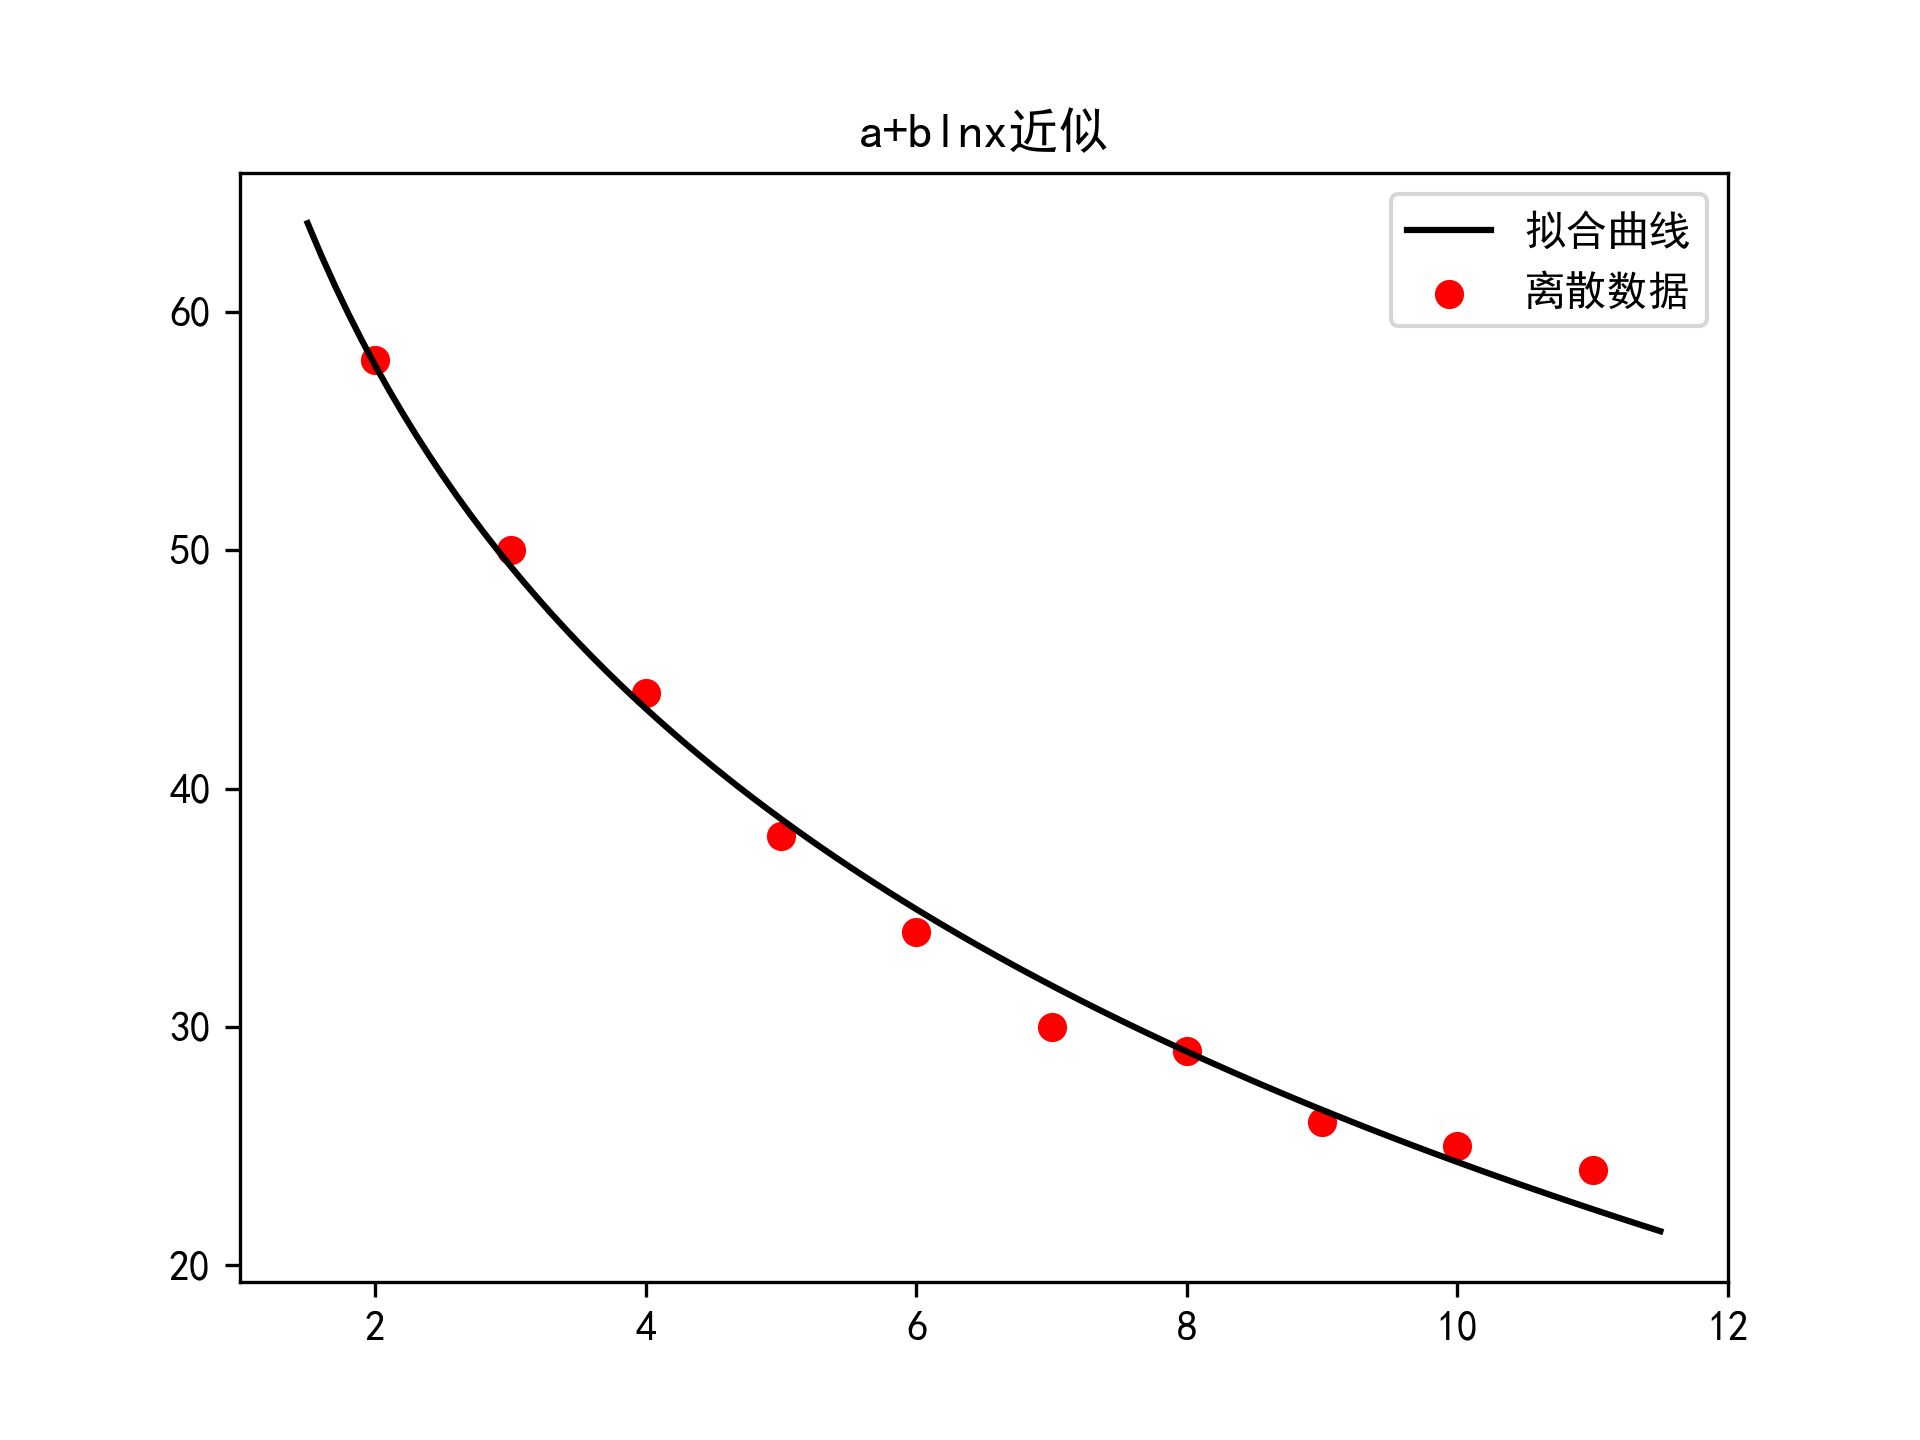
\includegraphics[width=\linewidth]{a+blnx近似}
        %\caption{fig2}
        \end{minipage}%
    }%

    \subfigure[$y=ae^{bx}$]{
        \begin{minipage}[t]{0.5\linewidth}
        \centering
        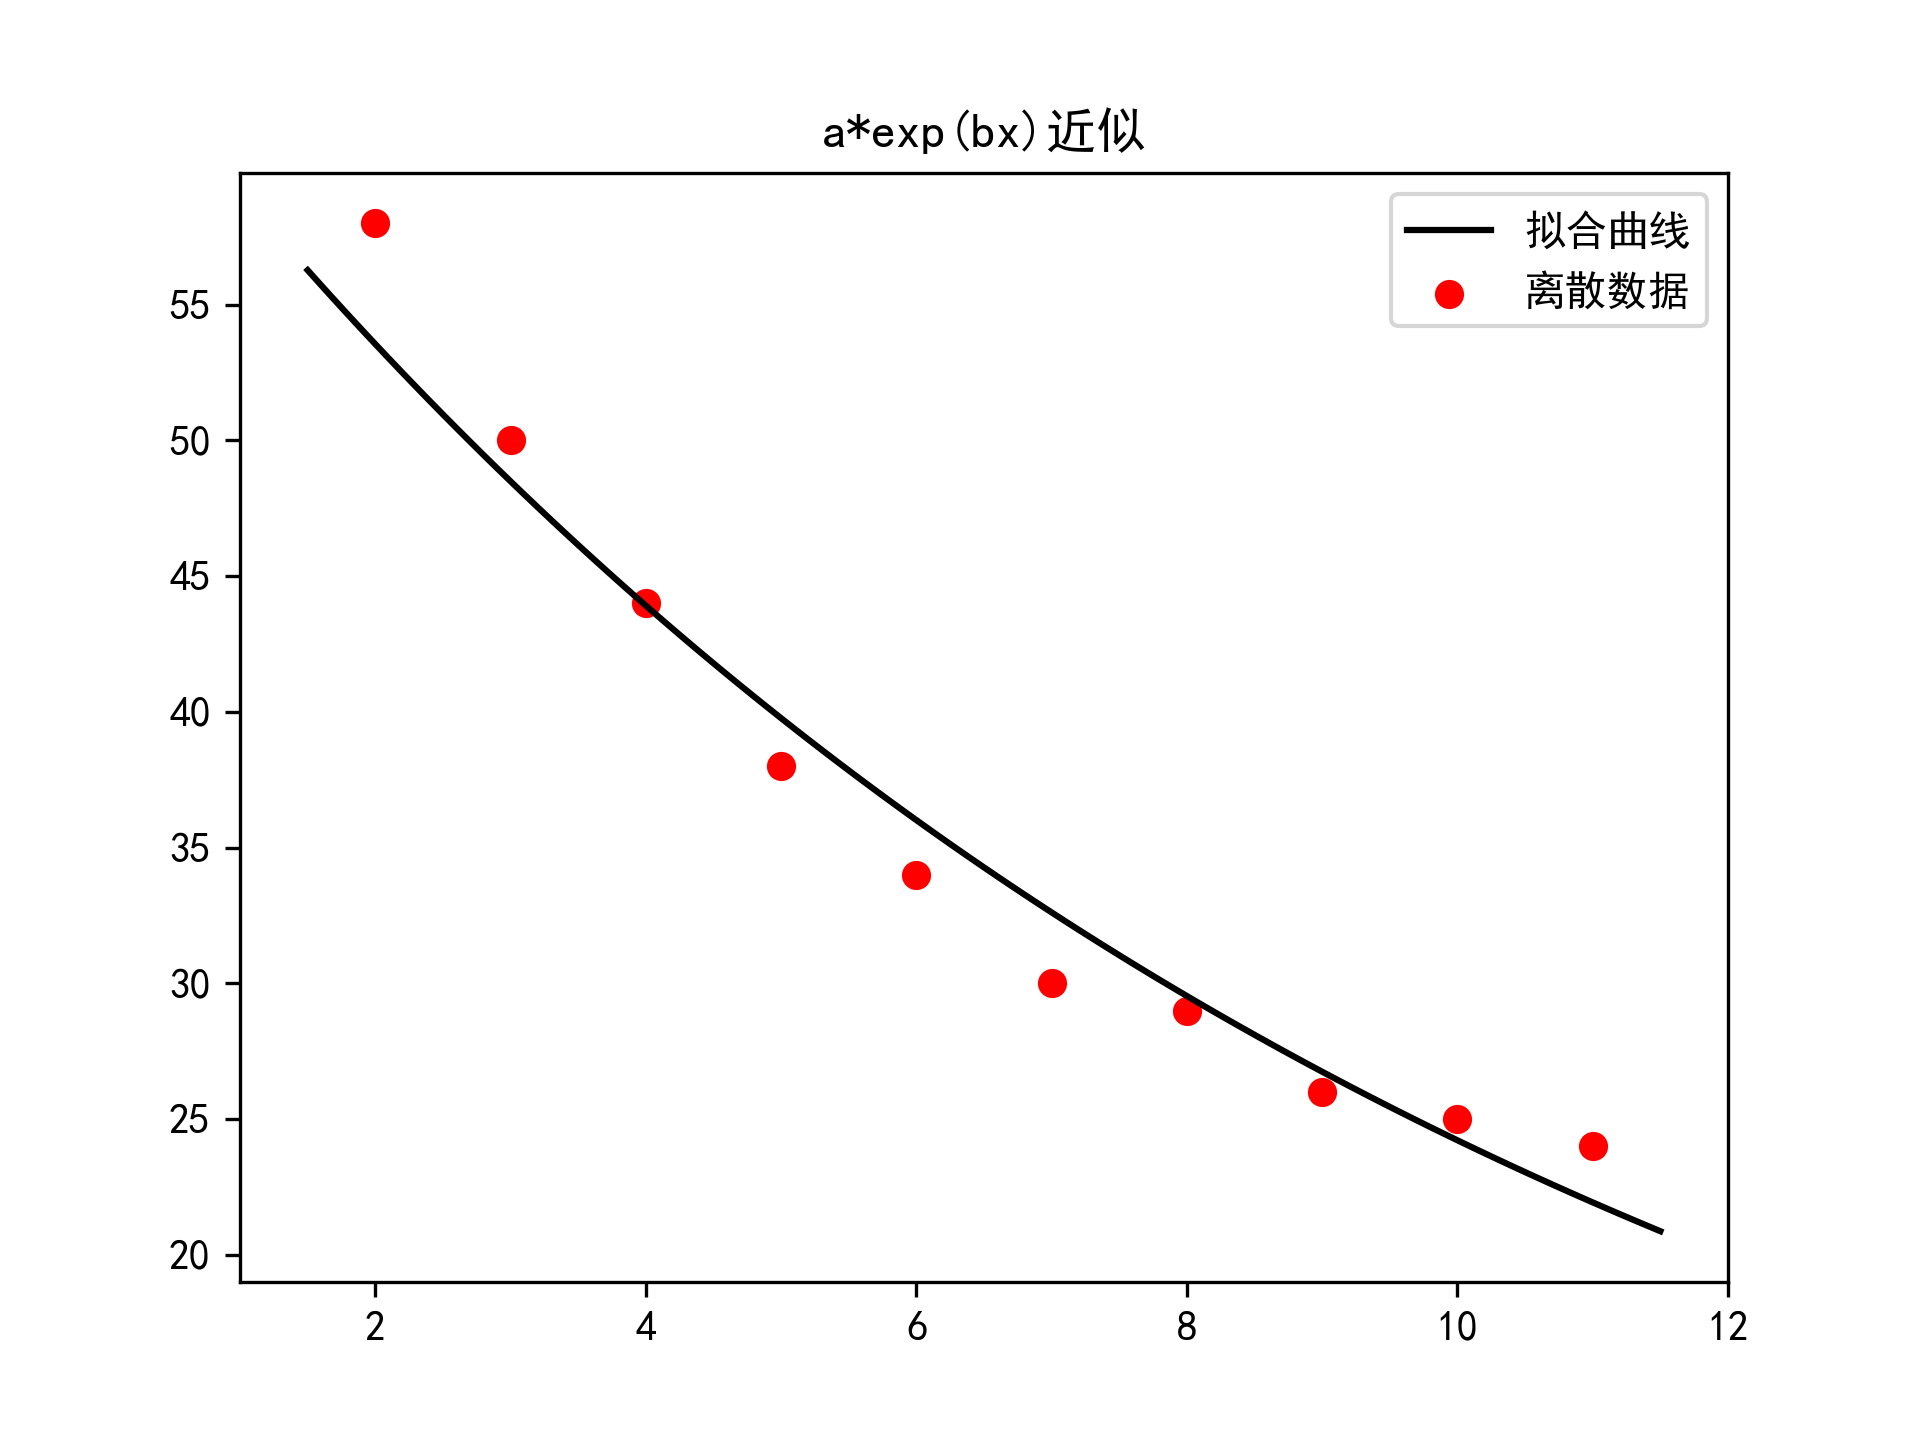
\includegraphics[width=\linewidth]{a*exp(bx)近似}
        %\caption{fig2}
        \end{minipage}
    }%
    \subfigure[$y={1}/(a+bx)$]{
        \begin{minipage}[t]{0.5\linewidth}
        \centering
        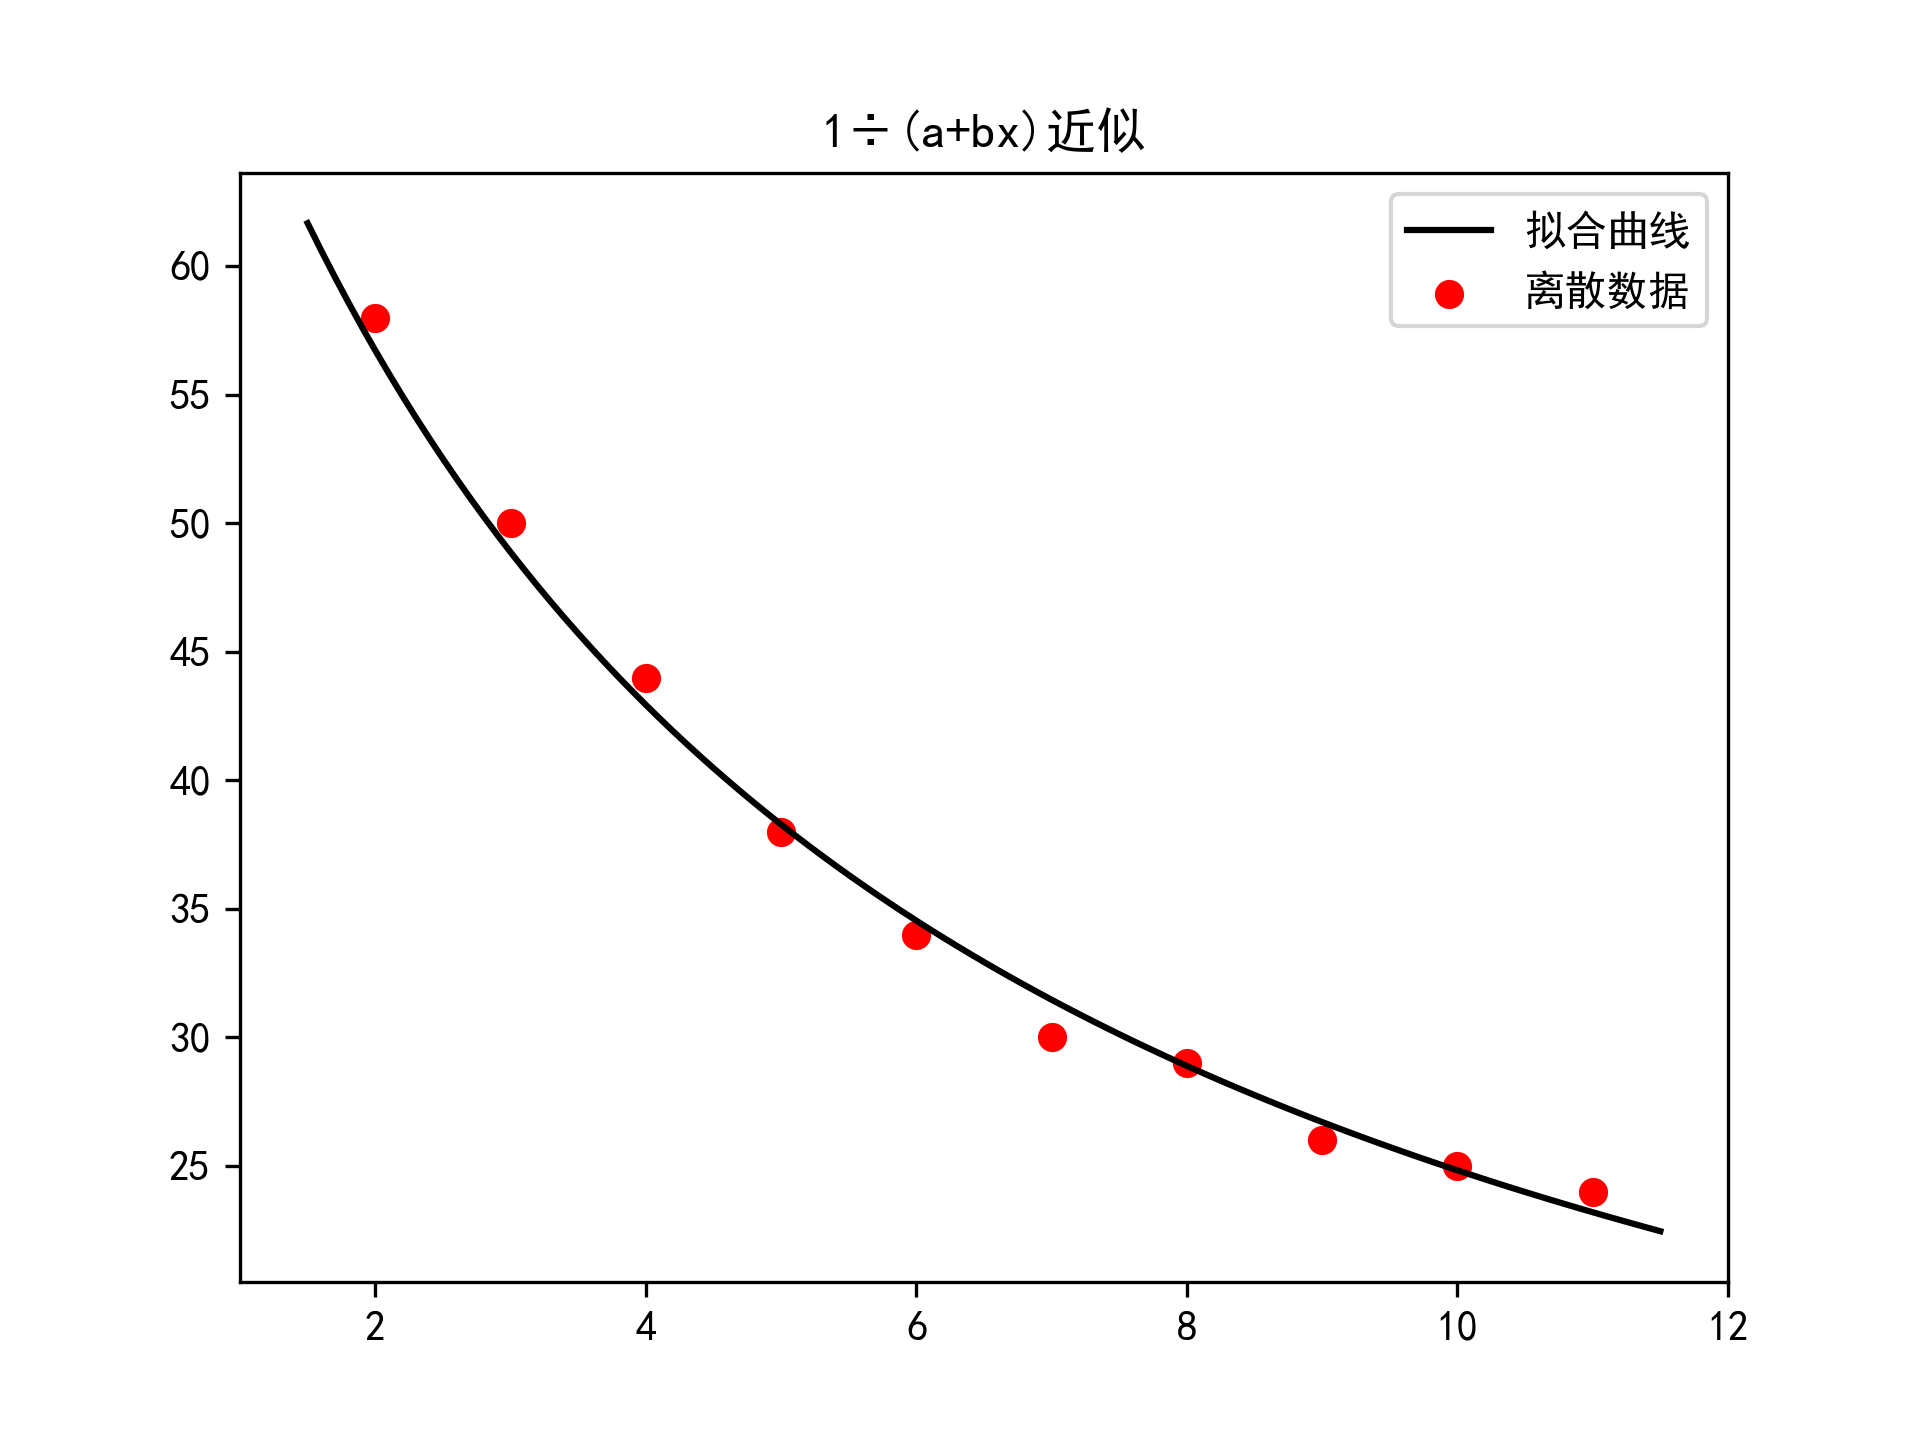
\includegraphics[width=\linewidth]{1÷(a+bx)近似}
        %\caption{fig2}
        \end{minipage}
    }%
    \centering
    \caption{最佳平方逼近变形}
    \label{fig:lsa2}
\end{figure}

\subsection{结论}

\begin{enumerate}[(1)]
    \item 7种不同的拟合函数的拟合误差对比如表\ref{tab:error}所示。通过对比可以看到4次最佳平方逼近的拟合误差最小,但也是计算量最大的一个。
    \item 4次最佳平方逼近的拟合误差相比于3次最佳平方逼近的拟合误差没有太多提升,反而加大了计算量。
    \item 在 4 种变形的拟合函数里,$y=a+b\mathrm{ln}x$ 和 $y={1}/(a+bx)$ 的闭合误差也比较小,但是都比2次最佳平方逼近的误差大。
    \item 整体上来说,相比于插值函数,次数不太高的最佳平方逼近的计算量不大。
\end{enumerate}

\begin{table}[ht]\centering
    \caption{拟合误差}
    \label{tab:error}
    \begin{tabular}{c|cccc}
        拟合函数 & 2次最佳平方逼近 & 3次最佳平方逼近 & 4次最佳平方逼近 & \\
        \hline
        拟合误差 & $3.2166667$ & $1.5102564$ & $1.4679487$ & \\
        \hline\hline
        拟合函数 & $y=a+{b}/{x}$ & $y=a+b\mathrm{ln}x$ & $y=ae^{bx}$ & $y={1}/(a+bx)$ \\
        \hline
        拟合误差 & $57.302270$ & $8.7788712$ & $41.844596$ & $7.7324292$
    \end{tabular}
\end{table}

% chapter chapter1 (end)